\documentclass[1p]{elsarticle_modified}
%\bibliographystyle{elsarticle-num}

%\usepackage[colorlinks]{hyperref}
%\usepackage{abbrmath_seonhwa} %\Abb, \Ascr, \Acal ,\Abf, \Afrak
\usepackage{amsfonts}
\usepackage{amssymb}
\usepackage{amsmath}
\usepackage{amsthm}
\usepackage{scalefnt}
\usepackage{amsbsy}
\usepackage{kotex}
\usepackage{caption}
\usepackage{subfig}
\usepackage{color}
\usepackage{graphicx}
\usepackage{xcolor} %% white, black, red, green, blue, cyan, magenta, yellow
\usepackage{float}
\usepackage{setspace}
\usepackage{hyperref}

\usepackage{tikz}
\usetikzlibrary{arrows}

\usepackage{multirow}
\usepackage{array} % fixed length table
\usepackage{hhline}

%%%%%%%%%%%%%%%%%%%%%
\makeatletter
\renewcommand*\env@matrix[1][\arraystretch]{%
	\edef\arraystretch{#1}%
	\hskip -\arraycolsep
	\let\@ifnextchar\new@ifnextchar
	\array{*\c@MaxMatrixCols c}}
\makeatother %https://tex.stackexchange.com/questions/14071/how-can-i-increase-the-line-spacing-in-a-matrix
%%%%%%%%%%%%%%%

\usepackage[normalem]{ulem}

\newcommand{\msout}[1]{\ifmmode\text{\sout{\ensuremath{#1}}}\else\sout{#1}\fi}
%SOURCE: \msout is \stkout macro in https://tex.stackexchange.com/questions/20609/strikeout-in-math-mode

\newcommand{\cancel}[1]{
	\ifmmode
	{\color{red}\msout{#1}}
	\else
	{\color{red}\sout{#1}}
	\fi
}

\newcommand{\add}[1]{
	{\color{blue}\uwave{#1}}
}

\newcommand{\replace}[2]{
	\ifmmode
	{\color{red}\msout{#1}}{\color{blue}\uwave{#2}}
	\else
	{\color{red}\sout{#1}}{\color{blue}\uwave{#2}}
	\fi
}

\newcommand{\Sol}{\mathcal{S}} %segment
\newcommand{\D}{D} %diagram
\newcommand{\A}{\mathcal{A}} %arc


%%%%%%%%%%%%%%%%%%%%%%%%%%%%%5 test

\def\sl{\operatorname{\textup{SL}}(2,\Cbb)}
\def\psl{\operatorname{\textup{PSL}}(2,\Cbb)}
\def\quan{\mkern 1mu \triangleright \mkern 1mu}

\theoremstyle{definition}
\newtheorem{thm}{Theorem}[section]
\newtheorem{prop}[thm]{Proposition}
\newtheorem{lem}[thm]{Lemma}
\newtheorem{ques}[thm]{Question}
\newtheorem{cor}[thm]{Corollary}
\newtheorem{defn}[thm]{Definition}
\newtheorem{exam}[thm]{Example}
\newtheorem{rmk}[thm]{Remark}
\newtheorem{alg}[thm]{Algorithm}

\newcommand{\I}{\sqrt{-1}}
\begin{document}

%\begin{frontmatter}
%
%\title{Boundary parabolic representations of knots up to 8 crossings}
%
%%% Group authors per affiliation:
%\author{Yunhi Cho} 
%\address{Department of Mathematics, University of Seoul, Seoul, Korea}
%\ead{yhcho@uos.ac.kr}
%
%
%\author{Seonhwa Kim} %\fnref{s_kim}}
%\address{Center for Geometry and Physics, Institute for Basic Science, Pohang, 37673, Korea}
%\ead{ryeona17@ibs.re.kr}
%
%\author{Hyuk Kim}
%\address{Department of Mathematical Sciences, Seoul National University, Seoul 08826, Korea}
%\ead{hyukkim@snu.ac.kr}
%
%\author{Seokbeom Yoon}
%\address{Department of Mathematical Sciences, Seoul National University, Seoul, 08826,  Korea}
%\ead{sbyoon15@snu.ac.kr}
%
%\begin{abstract}
%We find all boundary parabolic representation of knots up to 8 crossings.
%
%\end{abstract}
%\begin{keyword}
%    \MSC[2010] 57M25 
%\end{keyword}
%
%\end{frontmatter}

%\linenumbers
%\tableofcontents
%
\newcommand\colored[1]{\textcolor{white}{\rule[-0.35ex]{0.8em}{1.4ex}}\kern-0.8em\color{red} #1}%
%\newcommand\colored[1]{\textcolor{white}{ #1}\kern-2.17ex	\textcolor{white}{ #1}\kern-1.81ex	\textcolor{white}{ #1}\kern-2.15ex\color{red}#1	}

{\Large $\underline{11n_{76}~(K11n_{76})}$}

\setlength{\tabcolsep}{10pt}
\renewcommand{\arraystretch}{1.6}
\vspace{1cm}\begin{tabular}{m{100pt}>{\centering\arraybackslash}m{274pt}}
\multirow{5}{120pt}{
	\centering
	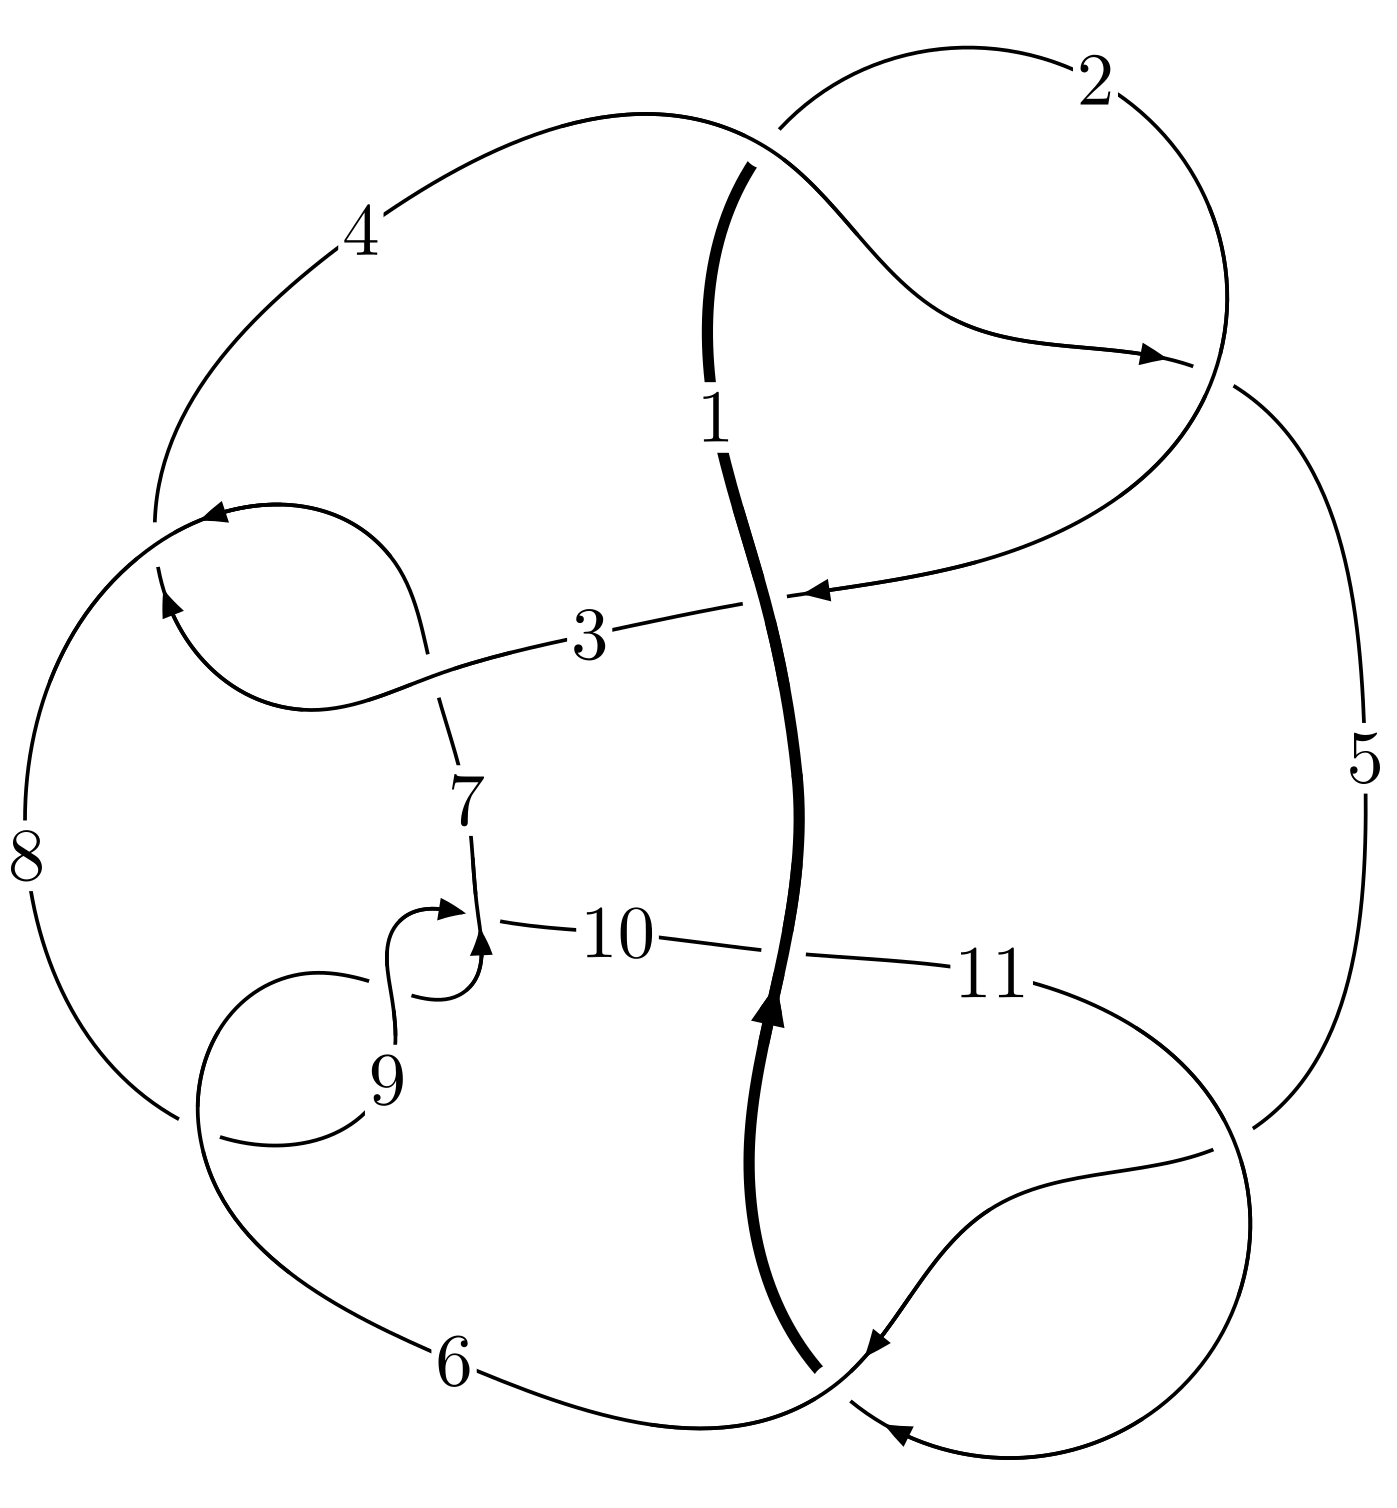
\includegraphics[width=112pt]{../../../GIT/diagram.site/Diagrams/png/692_11n_76.png}\\
\ \ \ A knot diagram\footnotemark}&
\allowdisplaybreaks
\textbf{Linearized knot diagam} \\
\cline{2-2}
 &
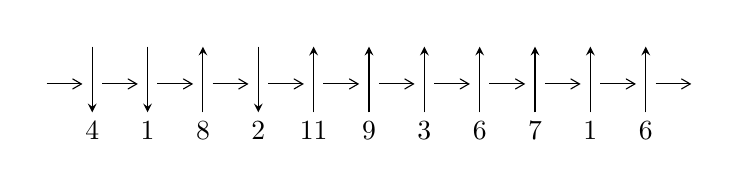
\begin{tikzpicture}[x=20pt, y=17pt]
	% nodes
	\node (C0) at (0, 0) {};
	\node (C1) at (1, 0) {};
	\node (C1U) at (1, +1) {};
	\node (C1D) at (1, -1) {4};

	\node (C2) at (2, 0) {};
	\node (C2U) at (2, +1) {};
	\node (C2D) at (2, -1) {1};

	\node (C3) at (3, 0) {};
	\node (C3U) at (3, +1) {};
	\node (C3D) at (3, -1) {8};

	\node (C4) at (4, 0) {};
	\node (C4U) at (4, +1) {};
	\node (C4D) at (4, -1) {2};

	\node (C5) at (5, 0) {};
	\node (C5U) at (5, +1) {};
	\node (C5D) at (5, -1) {11};

	\node (C6) at (6, 0) {};
	\node (C6U) at (6, +1) {};
	\node (C6D) at (6, -1) {9};

	\node (C7) at (7, 0) {};
	\node (C7U) at (7, +1) {};
	\node (C7D) at (7, -1) {3};

	\node (C8) at (8, 0) {};
	\node (C8U) at (8, +1) {};
	\node (C8D) at (8, -1) {6};

	\node (C9) at (9, 0) {};
	\node (C9U) at (9, +1) {};
	\node (C9D) at (9, -1) {7};

	\node (C10) at (10, 0) {};
	\node (C10U) at (10, +1) {};
	\node (C10D) at (10, -1) {1};

	\node (C11) at (11, 0) {};
	\node (C11U) at (11, +1) {};
	\node (C11D) at (11, -1) {6};
	\node (C12) at (12, 0) {};

	% arrows
	\draw[->,>={angle 60}]
	(C0) edge (C1) (C1) edge (C2) (C2) edge (C3) (C3) edge (C4) (C4) edge (C5) (C5) edge (C6) (C6) edge (C7) (C7) edge (C8) (C8) edge (C9) (C9) edge (C10) (C10) edge (C11) (C11) edge (C12) ;	\draw[->,>=stealth]
	(C1U) edge (C1D) (C2U) edge (C2D) (C3D) edge (C3U) (C4U) edge (C4D) (C5D) edge (C5U) (C6D) edge (C6U) (C7D) edge (C7U) (C8D) edge (C8U) (C9D) edge (C9U) (C10D) edge (C10U) (C11D) edge (C11U) ;
	\end{tikzpicture} \\
\hhline{~~} \\& 
\textbf{Solving Sequence} \\ \cline{2-2} 
 &
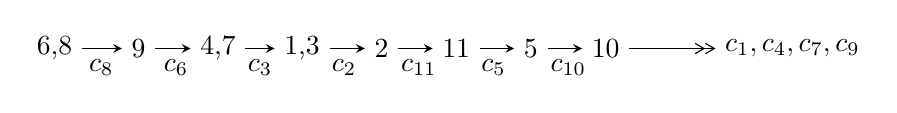
\begin{tikzpicture}[x=27pt, y=7pt]
	% node
	\node (A0) at (-1/8, 0) {6,8};
	\node (A1) at (1, 0) {9};
	\node (A2) at (33/16, 0) {4,7};
	\node (A3) at (51/16, 0) {1,3};
	\node (A4) at (17/4, 0) {2};
	\node (A5) at (21/4, 0) {11};
	\node (A6) at (25/4, 0) {5};
	\node (A7) at (29/4, 0) {10};
	\node (C1) at (1/2, -1) {$c_{8}$};
	\node (C2) at (3/2, -1) {$c_{6}$};
	\node (C3) at (21/8, -1) {$c_{3}$};
	\node (C4) at (15/4, -1) {$c_{2}$};
	\node (C5) at (19/4, -1) {$c_{11}$};
	\node (C6) at (23/4, -1) {$c_{5}$};
	\node (C7) at (27/4, -1) {$c_{10}$};
	\node (A8) at (39/4, 0) {$c_{1},c_{4},c_{7},c_{9}$};

	% edge
	\draw[->,>=stealth]	
	(A0) edge (A1) (A1) edge (A2) (A2) edge (A3) (A3) edge (A4) (A4) edge (A5) (A5) edge (A6) (A6) edge (A7) ;
	\draw[->>,>={angle 60}]	
	(A7) edge (A8);
\end{tikzpicture} \\ 

\end{tabular} \\

\footnotetext{
The image of knot diagram is generated by the software ``\textbf{Draw programme}" developed by Andrew Bartholomew(\url{http://www.layer8.co.uk/maths/draw/index.htm\#Running-draw}), where we modified some parts for our purpose(\url{https://github.com/CATsTAILs/LinksPainter}).
}\phantom \\ \newline 
\centering \textbf{Ideals for irreducible components\footnotemark of $X_{\text{par}}$} 
 
\begin{align*}
I^u_{1}&=\langle 
u^9+u^8-6 u^7-4 u^6+12 u^5+u^4-8 u^3+8 u^2+2 d- u,\\
\phantom{I^u_{1}}&\phantom{= \langle  }u^{10}+2 u^9-6 u^8-12 u^7+14 u^6+21 u^5-21 u^4-5 u^3+22 u^2+2 c-10 u,\\
\phantom{I^u_{1}}&\phantom{= \langle  }u^{10}+2 u^9-5 u^8-10 u^7+8 u^6+11 u^5-9 u^4+4 u^3+13 u^2+4 b+u,\;a-1,\\
\phantom{I^u_{1}}&\phantom{= \langle  }u^{11}+2 u^{10}-6 u^9-12 u^8+13 u^7+21 u^6-17 u^5-7 u^4+18 u^3-3 u^2- u-1\rangle \\
I^u_{2}&=\langle 
3 u^7+5 u^6-3 u^5- u^4+3 u^3-10 u^2+4 d-9 u-2,\;7 u^7+9 u^6-15 u^5- u^4+15 u^3-34 u^2+8 c-9 u+14,\\
\phantom{I^u_{2}}&\phantom{= \langle  }u^7+u^6- u^5+u^4+u^3-4 u^2+2 b-3 u,\;- u^7-3 u^6-3 u^5+3 u^4+3 u^3-6 u^2+8 a+7 u+18,\\
\phantom{I^u_{2}}&\phantom{= \langle  }u^8+u^7-3 u^6- u^5+3 u^4-4 u^3-3 u^2+4 u+4\rangle \\
I^u_{3}&=\langle 
d+u,\;c,\;- a u+b+a+1,\;a^2+a- u-1,\;u^2+u-1\rangle \\
I^u_{4}&=\langle 
u^3+d- u+1,\;u^3- u^2+c,\;u^3- u^2+b- u+2,\;- u^3+a-1,\;u^4- u^3+2 u-1\rangle \\
I^u_{5}&=\langle 
d+u,\;c,\;b+u+1,\;a-1,\;u^2+u-1\rangle \\
I^u_{6}&=\langle 
d,\;c+1,\;b,\;a+1,\;u-1\rangle \\
I^u_{7}&=\langle 
d,\;c-1,\;b+1,\;a,\;u-1\rangle \\
I^u_{8}&=\langle 
d,\;c b+1,\;a+1,\;u-1\rangle \\
\\
I^v_{1}&=\langle 
a,\;d,\;c-1,\;b+1,\;v-1\rangle \\
\end{align*}
\raggedright * 8 irreducible components of $\dim_{\mathbb{C}}=0$, with total 32 representations.\\
\raggedright * 1 irreducible components of $\dim_{\mathbb{C}}=1$ \\
\footnotetext{All coefficients of polynomials are rational numbers. But the coefficients are sometimes approximated in decimal forms when there is not enough margin.}
\newpage
\renewcommand{\arraystretch}{1}
\centering \section*{I. $I^u_{1}= \langle u^9+u^8+\cdots+2 d- u,\;u^{10}+2 u^9+\cdots+2 c-10 u,\;u^{10}+2 u^9+\cdots+4 b+u,\;a-1,\;u^{11}+2 u^{10}+\cdots- u-1 \rangle$}
\flushleft \textbf{(i) Arc colorings}\\
\begin{tabular}{m{7pt} m{180pt} m{7pt} m{180pt} }
\flushright $a_{6}=$&$\begin{pmatrix}0\\u\end{pmatrix}$ \\
\flushright $a_{8}=$&$\begin{pmatrix}1\\0\end{pmatrix}$ \\
\flushright $a_{9}=$&$\begin{pmatrix}1\\- u^2\end{pmatrix}$ \\
\flushright $a_{4}=$&$\begin{pmatrix}-\frac{1}{2} u^{10}- u^9+\cdots-11 u^2+5 u\\-\frac{1}{2} u^9-\frac{1}{2} u^8+\cdots-4 u^2+\frac{1}{2} u\end{pmatrix}$ \\
\flushright $a_{7}=$&$\begin{pmatrix}u\\- u^3+u\end{pmatrix}$ \\
\flushright $a_{1}=$&$\begin{pmatrix}1\\-\frac{1}{4} u^{10}-\frac{1}{2} u^9+\cdots-\frac{13}{4} u^2-\frac{1}{4} u\end{pmatrix}$ \\
\flushright $a_{3}=$&$\begin{pmatrix}-\frac{1}{2} u^{10}-\frac{1}{2} u^9+\cdots-7 u^2+\frac{9}{2} u\\-\frac{1}{2} u^9-\frac{1}{2} u^8+\cdots-4 u^2+\frac{1}{2} u\end{pmatrix}$ \\
\flushright $a_{2}=$&$\begin{pmatrix}-\frac{1}{2} u^{10}-\frac{3}{4} u^9+\cdots+\frac{19}{4} u+\frac{3}{4}\\-\frac{1}{2} u^{10}-\frac{3}{4} u^9+\cdots+\frac{3}{4} u+\frac{1}{4}\end{pmatrix}$ \\
\flushright $a_{11}=$&$\begin{pmatrix}1\\-\frac{1}{4} u^{10}-\frac{1}{2} u^9+\cdots-\frac{9}{4} u^2-\frac{1}{4} u\end{pmatrix}$ \\
\flushright $a_{5}=$&$\begin{pmatrix}- u\\\frac{1}{4} u^9+\frac{1}{2} u^8+\cdots+\frac{5}{4} u+\frac{1}{4}\end{pmatrix}$ \\
\flushright $a_{10}=$&$\begin{pmatrix}- u^2+1\\u^4-2 u^2\end{pmatrix}$\\ \flushright $a_{10}=$&$\begin{pmatrix}- u^2+1\\u^4-2 u^2\end{pmatrix}$\\&\end{tabular}
\flushleft \textbf{(ii) Obstruction class $= -1$}\\~\\
\flushleft \textbf{(iii) Cusp Shapes $= u^{10}+\frac{7}{2} u^9-4 u^8-\frac{45}{2} u^7+u^6+47 u^5+\frac{3}{2} u^4-\frac{71}{2} u^3+20 u^2+\frac{23}{2} u+\frac{1}{2}$}\\~\\
\newpage\renewcommand{\arraystretch}{1}
\flushleft \textbf{(iv) u-Polynomials at the component}\newline \\
\begin{tabular}{m{50pt}|m{274pt}}
Crossings & \hspace{64pt}u-Polynomials at each crossing \\
\hline $$\begin{aligned}c_{1},c_{4}\end{aligned}$$&$\begin{aligned}
&u^{11}-2 u^{10}+u^9+2 u^8-5 u^6+7 u^5+6 u^4-13 u^3+3 u^2+8 u-4
\end{aligned}$\\
\hline $$\begin{aligned}c_{2}\end{aligned}$$&$\begin{aligned}
&u^{11}+2 u^{10}+\cdots+88 u+16
\end{aligned}$\\
\hline $$\begin{aligned}c_{3},c_{7}\end{aligned}$$&$\begin{aligned}
&u^{11}+2 u^{10}- u^9-8 u^8-11 u^7+46 u^5+76 u^4+32 u^3-12 u^2-16 u-8
\end{aligned}$\\
\hline $$\begin{aligned}c_{5},c_{6},c_{8}\\c_{9},c_{11}\end{aligned}$$&$\begin{aligned}
&u^{11}+2 u^{10}+\cdots- u-1
\end{aligned}$\\
\hline $$\begin{aligned}c_{10}\end{aligned}$$&$\begin{aligned}
&u^{11}-16 u^{10}+\cdots-5 u-1
\end{aligned}$\\
\hline
\end{tabular}\\~\\
\newpage\renewcommand{\arraystretch}{1}
\flushleft \textbf{(v) Riley Polynomials at the component}\newline \\
\begin{tabular}{m{50pt}|m{274pt}}
Crossings & \hspace{64pt}Riley Polynomials at each crossing \\
\hline $$\begin{aligned}c_{1},c_{4}\end{aligned}$$&$\begin{aligned}
&y^{11}-2 y^{10}+\cdots+88 y-16
\end{aligned}$\\
\hline $$\begin{aligned}c_{2}\end{aligned}$$&$\begin{aligned}
&y^{11}+14 y^{10}+\cdots+2336 y-256
\end{aligned}$\\
\hline $$\begin{aligned}c_{3},c_{7}\end{aligned}$$&$\begin{aligned}
&y^{11}-6 y^{10}+\cdots+64 y-64
\end{aligned}$\\
\hline $$\begin{aligned}c_{5},c_{6},c_{8}\\c_{9},c_{11}\end{aligned}$$&$\begin{aligned}
&y^{11}-16 y^{10}+\cdots-5 y-1
\end{aligned}$\\
\hline $$\begin{aligned}c_{10}\end{aligned}$$&$\begin{aligned}
&y^{11}-36 y^{10}+\cdots-93 y-1
\end{aligned}$\\
\hline
\end{tabular}\\~\\
\newpage\flushleft \textbf{(vi) Complex Volumes and Cusp Shapes}
$$\begin{array}{c|c|c}  
\text{Solutions to }I^u_{1}& \I (\text{vol} + \sqrt{-1}CS) & \text{Cusp shape}\\
 \hline 
\begin{aligned}
u &= \phantom{-}0.552760 + 0.641799 I \\
a &= \phantom{-}1.00000\phantom{ +0.000000I} \\
b &= \phantom{-}0.82545 - 1.53098 I \\
c &= \phantom{-}0.712390 + 0.815288 I \\
d &= \phantom{-}1.044080 + 0.152224 I\end{aligned}
 & \phantom{-}0.79689 + 3.53286 I & \phantom{-}6.46290 - 7.08687 I \\ \hline\begin{aligned}
u &= \phantom{-}0.552760 - 0.641799 I \\
a &= \phantom{-}1.00000\phantom{ +0.000000I} \\
b &= \phantom{-}0.82545 + 1.53098 I \\
c &= \phantom{-}0.712390 - 0.815288 I \\
d &= \phantom{-}1.044080 - 0.152224 I\end{aligned}
 & \phantom{-}0.79689 - 3.53286 I & \phantom{-}6.46290 + 7.08687 I \\ \hline\begin{aligned}
u &= \phantom{-}0.590824\phantom{ +0.000000I} \\
a &= \phantom{-}1.00000\phantom{ +0.000000I} \\
b &= -1.42161\phantom{ +0.000000I} \\
c &= \phantom{-}0.0396568\phantom{ +0.000000I} \\
d &= -0.620148\phantom{ +0.000000I}\end{aligned}
 & \phantom{-}0.987118\phantom{ +0.000000I} & \phantom{-}9.97440\phantom{ +0.000000I} \\ \hline\begin{aligned}
u &= \phantom{-}1.64391 + 0.11631 I \\
a &= \phantom{-}1.00000\phantom{ +0.000000I} \\
b &= \phantom{-}0.437522 - 0.637453 I \\
c &= \phantom{-}0.234439 - 1.284060 I \\
d &= \phantom{-}0.24685 - 1.67120 I\end{aligned}
 & \phantom{-}10.83450 + 3.51232 I & \phantom{-}10.06687 - 2.29315 I \\ \hline\begin{aligned}
u &= \phantom{-}1.64391 - 0.11631 I \\
a &= \phantom{-}1.00000\phantom{ +0.000000I} \\
b &= \phantom{-}0.437522 + 0.637453 I \\
c &= \phantom{-}0.234439 + 1.284060 I \\
d &= \phantom{-}0.24685 + 1.67120 I\end{aligned}
 & \phantom{-}10.83450 - 3.51232 I & \phantom{-}10.06687 + 2.29315 I \\ \hline\begin{aligned}
u &= -1.60901 + 0.41639 I \\
a &= \phantom{-}1.00000\phantom{ +0.000000I} \\
b &= \phantom{-}0.32965 + 2.04536 I \\
c &= \phantom{-}0.194428 - 1.371430 I \\
d &= \phantom{-}1.57467 - 0.87175 I\end{aligned}
 & \phantom{-}14.9243 - 12.3125 I & \phantom{-}9.62929 + 5.75829 I\\
 \hline 
 \end{array}$$\newpage$$\begin{array}{c|c|c}  
\text{Solutions to }I^u_{1}& \I (\text{vol} + \sqrt{-1}CS) & \text{Cusp shape}\\
 \hline 
\begin{aligned}
u &= -1.60901 - 0.41639 I \\
a &= \phantom{-}1.00000\phantom{ +0.000000I} \\
b &= \phantom{-}0.32965 - 2.04536 I \\
c &= \phantom{-}0.194428 + 1.371430 I \\
d &= \phantom{-}1.57467 + 0.87175 I\end{aligned}
 & \phantom{-}14.9243 + 12.3125 I & \phantom{-}9.62929 - 5.75829 I \\ \hline\begin{aligned}
u &= -0.162723 + 0.277330 I \\
a &= \phantom{-}1.00000\phantom{ +0.000000I} \\
b &= \phantom{-}0.160409 + 0.252652 I \\
c &= -0.22673 + 2.50982 I \\
d &= \phantom{-}0.267436 + 0.517187 I\end{aligned}
 & -1.66390 - 0.61823 I & -3.63835 + 1.22407 I \\ \hline\begin{aligned}
u &= -0.162723 - 0.277330 I \\
a &= \phantom{-}1.00000\phantom{ +0.000000I} \\
b &= \phantom{-}0.160409 - 0.252652 I \\
c &= -0.22673 - 2.50982 I \\
d &= \phantom{-}0.267436 - 0.517187 I\end{aligned}
 & -1.66390 + 0.61823 I & -3.63835 - 1.22407 I \\ \hline\begin{aligned}
u &= -1.72035 + 0.28600 I \\
a &= \phantom{-}1.00000\phantom{ +0.000000I} \\
b &= -0.04222 + 1.42193 I \\
c &= -0.434360 + 0.920646 I \\
d &= -1.82296 + 0.61164 I\end{aligned}
 & \phantom{-}17.3830 - 4.9116 I & \phantom{-}11.49209 + 1.65700 I \\ \hline\begin{aligned}
u &= -1.72035 - 0.28600 I \\
a &= \phantom{-}1.00000\phantom{ +0.000000I} \\
b &= -0.04222 - 1.42193 I \\
c &= -0.434360 - 0.920646 I \\
d &= -1.82296 - 0.61164 I\end{aligned}
 & \phantom{-}17.3830 + 4.9116 I & \phantom{-}11.49209 - 1.65700 I\\
 \hline 
 \end{array}$$\newpage\newpage\renewcommand{\arraystretch}{1}
\centering \section*{II. $I^u_{2}= \langle 3 u^7+5 u^6+\cdots+4 d-2,\;7 u^7+9 u^6+\cdots+8 c+14,\;u^7+u^6+\cdots+2 b-3 u,\;- u^7-3 u^6+\cdots+8 a+18,\;u^8+u^7+\cdots+4 u+4 \rangle$}
\flushleft \textbf{(i) Arc colorings}\\
\begin{tabular}{m{7pt} m{180pt} m{7pt} m{180pt} }
\flushright $a_{6}=$&$\begin{pmatrix}0\\u\end{pmatrix}$ \\
\flushright $a_{8}=$&$\begin{pmatrix}1\\0\end{pmatrix}$ \\
\flushright $a_{9}=$&$\begin{pmatrix}1\\- u^2\end{pmatrix}$ \\
\flushright $a_{4}=$&$\begin{pmatrix}-\frac{7}{8} u^7-\frac{9}{8} u^6+\cdots+\frac{9}{8} u-\frac{7}{4}\\-\frac{3}{4} u^7-\frac{5}{4} u^6+\cdots+\frac{9}{4} u+\frac{1}{2}\end{pmatrix}$ \\
\flushright $a_{7}=$&$\begin{pmatrix}u\\- u^3+u\end{pmatrix}$ \\
\flushright $a_{1}=$&$\begin{pmatrix}\frac{1}{8} u^7+\frac{3}{8} u^6+\cdots-\frac{7}{8} u-\frac{9}{4}\\-\frac{1}{2} u^7-\frac{1}{2} u^6+\cdots+2 u^2+\frac{3}{2} u\end{pmatrix}$ \\
\flushright $a_{3}=$&$\begin{pmatrix}-\frac{1}{8} u^7+\frac{1}{8} u^6+\cdots-\frac{9}{8} u-\frac{9}{4}\\-\frac{3}{4} u^7-\frac{5}{4} u^6+\cdots+\frac{9}{4} u+\frac{1}{2}\end{pmatrix}$ \\
\flushright $a_{2}=$&$\begin{pmatrix}-\frac{1}{2} u^7+2 u^5+\cdots-\frac{1}{2} u-\frac{5}{2}\\-\frac{3}{4} u^7-\frac{5}{4} u^6+\cdots+\frac{13}{4} u+\frac{3}{2}\end{pmatrix}$ \\
\flushright $a_{11}=$&$\begin{pmatrix}\frac{1}{8} u^7+\frac{3}{8} u^6+\cdots-\frac{7}{8} u-\frac{9}{4}\\-1\end{pmatrix}$ \\
\flushright $a_{5}=$&$\begin{pmatrix}\frac{1}{2} u^7+u^6+\cdots-\frac{5}{2} u+\frac{1}{2}\\\frac{1}{4} u^7+\frac{3}{4} u^6+\cdots-\frac{7}{4} u-\frac{1}{2}\end{pmatrix}$ \\
\flushright $a_{10}=$&$\begin{pmatrix}- u^2+1\\u^4-2 u^2\end{pmatrix}$\\ \flushright $a_{10}=$&$\begin{pmatrix}- u^2+1\\u^4-2 u^2\end{pmatrix}$\\&\end{tabular}
\flushleft \textbf{(ii) Obstruction class $= -1$}\\~\\
\flushleft \textbf{(iii) Cusp Shapes $= 4 u^7+6 u^6-4 u^5+6 u^3-14 u^2-14 u+4$}\\~\\
\newpage\renewcommand{\arraystretch}{1}
\flushleft \textbf{(iv) u-Polynomials at the component}\newline \\
\begin{tabular}{m{50pt}|m{274pt}}
Crossings & \hspace{64pt}u-Polynomials at each crossing \\
\hline $$\begin{aligned}c_{1},c_{4}\end{aligned}$$&$\begin{aligned}
&(u^4- u^3+u+1)^2
\end{aligned}$\\
\hline $$\begin{aligned}c_{2}\end{aligned}$$&$\begin{aligned}
&(u^4+u^3+4 u^2+u+1)^2
\end{aligned}$\\
\hline $$\begin{aligned}c_{3},c_{7}\end{aligned}$$&$\begin{aligned}
&(u^4-3 u^3+3 u^2-2 u+2)^2
\end{aligned}$\\
\hline $$\begin{aligned}c_{5},c_{6},c_{8}\\c_{9},c_{11}\end{aligned}$$&$\begin{aligned}
&u^8+u^7-3 u^6- u^5+3 u^4-4 u^3-3 u^2+4 u+4
\end{aligned}$\\
\hline $$\begin{aligned}c_{10}\end{aligned}$$&$\begin{aligned}
&u^8-7 u^7+17 u^6-17 u^5+19 u^4-50 u^3+65 u^2-40 u+16
\end{aligned}$\\
\hline
\end{tabular}\\~\\
\newpage\renewcommand{\arraystretch}{1}
\flushleft \textbf{(v) Riley Polynomials at the component}\newline \\
\begin{tabular}{m{50pt}|m{274pt}}
Crossings & \hspace{64pt}Riley Polynomials at each crossing \\
\hline $$\begin{aligned}c_{1},c_{4}\end{aligned}$$&$\begin{aligned}
&(y^4- y^3+4 y^2- y+1)^2
\end{aligned}$\\
\hline $$\begin{aligned}c_{2}\end{aligned}$$&$\begin{aligned}
&(y^4+7 y^3+16 y^2+7 y+1)^2
\end{aligned}$\\
\hline $$\begin{aligned}c_{3},c_{7}\end{aligned}$$&$\begin{aligned}
&(y^4-3 y^3+y^2+8 y+4)^2
\end{aligned}$\\
\hline $$\begin{aligned}c_{5},c_{6},c_{8}\\c_{9},c_{11}\end{aligned}$$&$\begin{aligned}
&y^8-7 y^7+17 y^6-17 y^5+19 y^4-50 y^3+65 y^2-40 y+16
\end{aligned}$\\
\hline $$\begin{aligned}c_{10}\end{aligned}$$&$\begin{aligned}
&y^8-15 y^7+89 y^6-213 y^5+343 y^4-846 y^3+833 y^2+480 y+256
\end{aligned}$\\
\hline
\end{tabular}\\~\\
\newpage\flushleft \textbf{(vi) Complex Volumes and Cusp Shapes}
$$\begin{array}{c|c|c}  
\text{Solutions to }I^u_{2}& \I (\text{vol} + \sqrt{-1}CS) & \text{Cusp shape}\\
 \hline 
\begin{aligned}
u &= -0.695289 + 0.428533 I \\
a &= -1.29532 - 0.84192 I \\
b &= -0.109976 - 0.519497 I \\
c &= -0.57622 - 2.77692 I \\
d &= \phantom{-}0.066121 - 0.864054 I\end{aligned}
 & \phantom{-}2.62917 - 1.45022 I & \phantom{-}7.43990 + 4.72374 I \\ \hline\begin{aligned}
u &= -0.695289 - 0.428533 I \\
a &= -1.29532 + 0.84192 I \\
b &= -0.109976 + 0.519497 I \\
c &= -0.57622 + 2.77692 I \\
d &= \phantom{-}0.066121 + 0.864054 I\end{aligned}
 & \phantom{-}2.62917 + 1.45022 I & \phantom{-}7.43990 - 4.72374 I \\ \hline\begin{aligned}
u &= \phantom{-}0.529919 + 1.081980 I \\
a &= -0.745137 + 1.110160 I \\
b &= -0.39002 + 1.84237 I \\
c &= -1.47609 - 1.17606 I \\
d &= -1.56612 - 0.45882 I\end{aligned}
 & \phantom{-}8.06290 + 6.78371 I & \phantom{-}8.56010 - 4.72374 I \\ \hline\begin{aligned}
u &= \phantom{-}0.529919 - 1.081980 I \\
a &= -0.745137 - 1.110160 I \\
b &= -0.39002 - 1.84237 I \\
c &= -1.47609 + 1.17606 I \\
d &= -1.56612 + 0.45882 I\end{aligned}
 & \phantom{-}8.06290 - 6.78371 I & \phantom{-}8.56010 + 4.72374 I \\ \hline\begin{aligned}
u &= \phantom{-}1.261410 + 0.030288 I \\
a &= -0.542730 + 0.352757 I \\
b &= -0.109976 - 0.519497 I \\
c &= \phantom{-}0.054288 - 0.560610 I \\
d &= \phantom{-}0.066121 - 0.864054 I\end{aligned}
 & \phantom{-}2.62917 - 1.45022 I & \phantom{-}7.43990 + 4.72374 I \\ \hline\begin{aligned}
u &= \phantom{-}1.261410 - 0.030288 I \\
a &= -0.542730 - 0.352757 I \\
b &= -0.109976 + 0.519497 I \\
c &= \phantom{-}0.054288 + 0.560610 I \\
d &= \phantom{-}0.066121 + 0.864054 I\end{aligned}
 & \phantom{-}2.62917 + 1.45022 I & \phantom{-}7.43990 - 4.72374 I\\
 \hline 
 \end{array}$$\newpage$$\begin{array}{c|c|c}  
\text{Solutions to }I^u_{2}& \I (\text{vol} + \sqrt{-1}CS) & \text{Cusp shape}\\
 \hline 
\begin{aligned}
u &= -1.59604 + 0.21793 I \\
a &= -0.416815 + 0.621004 I \\
b &= -0.39002 - 1.84237 I \\
c &= -0.001980 + 0.777911 I \\
d &= -1.56612 + 0.45882 I\end{aligned}
 & \phantom{-}8.06290 - 6.78371 I & \phantom{-}8.56010 + 4.72374 I \\ \hline\begin{aligned}
u &= -1.59604 - 0.21793 I \\
a &= -0.416815 - 0.621004 I \\
b &= -0.39002 + 1.84237 I \\
c &= -0.001980 - 0.777911 I \\
d &= -1.56612 - 0.45882 I\end{aligned}
 & \phantom{-}8.06290 + 6.78371 I & \phantom{-}8.56010 - 4.72374 I\\
 \hline 
 \end{array}$$\newpage\newpage\renewcommand{\arraystretch}{1}
\centering \section*{III. $I^u_{3}= \langle d+u,\;c,\;- a u+b+a+1,\;a^2+a- u-1,\;u^2+u-1 \rangle$}
\flushleft \textbf{(i) Arc colorings}\\
\begin{tabular}{m{7pt} m{180pt} m{7pt} m{180pt} }
\flushright $a_{6}=$&$\begin{pmatrix}0\\u\end{pmatrix}$ \\
\flushright $a_{8}=$&$\begin{pmatrix}1\\0\end{pmatrix}$ \\
\flushright $a_{9}=$&$\begin{pmatrix}1\\u-1\end{pmatrix}$ \\
\flushright $a_{4}=$&$\begin{pmatrix}0\\- u\end{pmatrix}$ \\
\flushright $a_{7}=$&$\begin{pmatrix}u\\- u+1\end{pmatrix}$ \\
\flushright $a_{1}=$&$\begin{pmatrix}a\\a u- a-1\end{pmatrix}$ \\
\flushright $a_{3}=$&$\begin{pmatrix}u\\- u\end{pmatrix}$ \\
\flushright $a_{2}=$&$\begin{pmatrix}a\\-1\end{pmatrix}$ \\
\flushright $a_{11}=$&$\begin{pmatrix}a\\-1\end{pmatrix}$ \\
\flushright $a_{5}=$&$\begin{pmatrix}a u-1\\a u+u\end{pmatrix}$ \\
\flushright $a_{10}=$&$\begin{pmatrix}u\\- u\end{pmatrix}$\\ \flushright $a_{10}=$&$\begin{pmatrix}u\\- u\end{pmatrix}$\\&\end{tabular}
\flushleft \textbf{(ii) Obstruction class $= -1$}\\~\\
\flushleft \textbf{(iii) Cusp Shapes $= 10$}\\~\\
\newpage\renewcommand{\arraystretch}{1}
\flushleft \textbf{(iv) u-Polynomials at the component}\newline \\
\begin{tabular}{m{50pt}|m{274pt}}
Crossings & \hspace{64pt}u-Polynomials at each crossing \\
\hline $$\begin{aligned}c_{1},c_{4},c_{5}\\c_{11}\end{aligned}$$&$\begin{aligned}
&u^4- u^3+2 u-1
\end{aligned}$\\
\hline $$\begin{aligned}c_{2}\end{aligned}$$&$\begin{aligned}
&u^4+u^3+2 u^2+4 u+1
\end{aligned}$\\
\hline $$\begin{aligned}c_{3},c_{6},c_{7}\\c_{8},c_{9}\end{aligned}$$&$\begin{aligned}
&(u^2+u-1)^2
\end{aligned}$\\
\hline $$\begin{aligned}c_{10}\end{aligned}$$&$\begin{aligned}
&u^4- u^3+2 u^2-4 u+1
\end{aligned}$\\
\hline
\end{tabular}\\~\\
\newpage\renewcommand{\arraystretch}{1}
\flushleft \textbf{(v) Riley Polynomials at the component}\newline \\
\begin{tabular}{m{50pt}|m{274pt}}
Crossings & \hspace{64pt}Riley Polynomials at each crossing \\
\hline $$\begin{aligned}c_{1},c_{4},c_{5}\\c_{11}\end{aligned}$$&$\begin{aligned}
&y^4- y^3+2 y^2-4 y+1
\end{aligned}$\\
\hline $$\begin{aligned}c_{2},c_{10}\end{aligned}$$&$\begin{aligned}
&y^4+3 y^3-2 y^2-12 y+1
\end{aligned}$\\
\hline $$\begin{aligned}c_{3},c_{6},c_{7}\\c_{8},c_{9}\end{aligned}$$&$\begin{aligned}
&(y^2-3 y+1)^2
\end{aligned}$\\
\hline
\end{tabular}\\~\\
\newpage\flushleft \textbf{(vi) Complex Volumes and Cusp Shapes}
$$\begin{array}{c|c|c}  
\text{Solutions to }I^u_{3}& \I (\text{vol} + \sqrt{-1}CS) & \text{Cusp shape}\\
 \hline 
\begin{aligned}
u &= \phantom{-}0.618034\phantom{ +0.000000I} \\
a &= \phantom{-}0.866760\phantom{ +0.000000I} \\
b &= -1.33107\phantom{ +0.000000I} \\
c &= \phantom{-0.000000 } 0 \\
d &= -0.618034\phantom{ +0.000000I}\end{aligned}
 & \phantom{-}0.986960\phantom{ +0.000000I} & \phantom{-}10.0000\phantom{ +0.000000I} \\ \hline\begin{aligned}
u &= \phantom{-}0.618034\phantom{ +0.000000I} \\
a &= -1.86676\phantom{ +0.000000I} \\
b &= -0.286961\phantom{ +0.000000I} \\
c &= \phantom{-0.000000 } 0 \\
d &= -0.618034\phantom{ +0.000000I}\end{aligned}
 & \phantom{-}0.986960\phantom{ +0.000000I} & \phantom{-}10.0000\phantom{ +0.000000I} \\ \hline\begin{aligned}
u &= -1.61803\phantom{ +0.000000I} \\
a &= -0.500000 + 0.606658 I \\
b &= \phantom{-}0.30902 - 1.58825 I \\
c &= \phantom{-0.000000 } 0 \\
d &= \phantom{-}1.61803\phantom{ +0.000000I}\end{aligned}
 & \phantom{-}8.88264\phantom{ +0.000000I} & \phantom{-}10.0000\phantom{ +0.000000I} \\ \hline\begin{aligned}
u &= -1.61803\phantom{ +0.000000I} \\
a &= -0.500000 - 0.606658 I \\
b &= \phantom{-}0.30902 + 1.58825 I \\
c &= \phantom{-0.000000 } 0 \\
d &= \phantom{-}1.61803\phantom{ +0.000000I}\end{aligned}
 & \phantom{-}8.88264\phantom{ +0.000000I} & \phantom{-}10.0000\phantom{ +0.000000I}\\
 \hline 
 \end{array}$$\newpage\newpage\renewcommand{\arraystretch}{1}
\centering \section*{IV. $I^u_{4}= \langle u^3+d- u+1,\;u^3- u^2+c,\;u^3- u^2+b- u+2,\;- u^3+a-1,\;u^4- u^3+2 u-1 \rangle$}
\flushleft \textbf{(i) Arc colorings}\\
\begin{tabular}{m{7pt} m{180pt} m{7pt} m{180pt} }
\flushright $a_{6}=$&$\begin{pmatrix}0\\u\end{pmatrix}$ \\
\flushright $a_{8}=$&$\begin{pmatrix}1\\0\end{pmatrix}$ \\
\flushright $a_{9}=$&$\begin{pmatrix}1\\- u^2\end{pmatrix}$ \\
\flushright $a_{4}=$&$\begin{pmatrix}- u^3+u^2\\- u^3+u-1\end{pmatrix}$ \\
\flushright $a_{7}=$&$\begin{pmatrix}u\\- u^3+u\end{pmatrix}$ \\
\flushright $a_{1}=$&$\begin{pmatrix}u^3+1\\- u^3+u^2+u-2\end{pmatrix}$ \\
\flushright $a_{3}=$&$\begin{pmatrix}u^2- u+1\\- u^3+u-1\end{pmatrix}$ \\
\flushright $a_{2}=$&$\begin{pmatrix}u^3-2 u+2\\-1\end{pmatrix}$ \\
\flushright $a_{11}=$&$\begin{pmatrix}u^3+1\\-1\end{pmatrix}$ \\
\flushright $a_{5}=$&$\begin{pmatrix}u^2-1\\u^3+1\end{pmatrix}$ \\
\flushright $a_{10}=$&$\begin{pmatrix}- u^2+1\\u^3-2 u^2-2 u+1\end{pmatrix}$\\ \flushright $a_{10}=$&$\begin{pmatrix}- u^2+1\\u^3-2 u^2-2 u+1\end{pmatrix}$\\&\end{tabular}
\flushleft \textbf{(ii) Obstruction class $= -1$}\\~\\
\flushleft \textbf{(iii) Cusp Shapes $= 10$}\\~\\
\newpage\renewcommand{\arraystretch}{1}
\flushleft \textbf{(iv) u-Polynomials at the component}\newline \\
\begin{tabular}{m{50pt}|m{274pt}}
Crossings & \hspace{64pt}u-Polynomials at each crossing \\
\hline $$\begin{aligned}c_{1},c_{4},c_{6}\\c_{8},c_{9}\end{aligned}$$&$\begin{aligned}
&u^4- u^3+2 u-1
\end{aligned}$\\
\hline $$\begin{aligned}c_{2}\end{aligned}$$&$\begin{aligned}
&u^4+u^3+2 u^2+4 u+1
\end{aligned}$\\
\hline $$\begin{aligned}c_{3},c_{5},c_{7}\\c_{11}\end{aligned}$$&$\begin{aligned}
&(u^2+u-1)^2
\end{aligned}$\\
\hline $$\begin{aligned}c_{10}\end{aligned}$$&$\begin{aligned}
&(u^2-3 u+1)^2
\end{aligned}$\\
\hline
\end{tabular}\\~\\
\newpage\renewcommand{\arraystretch}{1}
\flushleft \textbf{(v) Riley Polynomials at the component}\newline \\
\begin{tabular}{m{50pt}|m{274pt}}
Crossings & \hspace{64pt}Riley Polynomials at each crossing \\
\hline $$\begin{aligned}c_{1},c_{4},c_{6}\\c_{8},c_{9}\end{aligned}$$&$\begin{aligned}
&y^4- y^3+2 y^2-4 y+1
\end{aligned}$\\
\hline $$\begin{aligned}c_{2}\end{aligned}$$&$\begin{aligned}
&y^4+3 y^3-2 y^2-12 y+1
\end{aligned}$\\
\hline $$\begin{aligned}c_{3},c_{5},c_{7}\\c_{11}\end{aligned}$$&$\begin{aligned}
&(y^2-3 y+1)^2
\end{aligned}$\\
\hline $$\begin{aligned}c_{10}\end{aligned}$$&$\begin{aligned}
&(y^2-7 y+1)^2
\end{aligned}$\\
\hline
\end{tabular}\\~\\
\newpage\flushleft \textbf{(vi) Complex Volumes and Cusp Shapes}
$$\begin{array}{c|c|c}  
\text{Solutions to }I^u_{4}& \I (\text{vol} + \sqrt{-1}CS) & \text{Cusp shape}\\
 \hline 
\begin{aligned}
u &= -1.15372\phantom{ +0.000000I} \\
a &= -0.535687\phantom{ +0.000000I} \\
b &= -0.286961\phantom{ +0.000000I} \\
c &= \phantom{-}2.86676\phantom{ +0.000000I} \\
d &= -0.618034\phantom{ +0.000000I}\end{aligned}
 & \phantom{-}0.986960\phantom{ +0.000000I} & \phantom{-}10.0000\phantom{ +0.000000I} \\ \hline\begin{aligned}
u &= \phantom{-}0.809017 + 0.981593 I \\
a &= -0.809017 + 0.981593 I \\
b &= \phantom{-}0.30902 + 1.58825 I \\
c &= \phantom{-}1.50000 + 0.60666 I \\
d &= \phantom{-}1.61803\phantom{ +0.000000I}\end{aligned}
 & \phantom{-}8.88264\phantom{ +0.000000I} & \phantom{-}10.0000\phantom{ +0.000000I} \\ \hline\begin{aligned}
u &= \phantom{-}0.809017 - 0.981593 I \\
a &= -0.809017 - 0.981593 I \\
b &= \phantom{-}0.30902 - 1.58825 I \\
c &= \phantom{-}1.50000 - 0.60666 I \\
d &= \phantom{-}1.61803\phantom{ +0.000000I}\end{aligned}
 & \phantom{-}8.88264\phantom{ +0.000000I} & \phantom{-}10.0000\phantom{ +0.000000I} \\ \hline\begin{aligned}
u &= \phantom{-}0.535687\phantom{ +0.000000I} \\
a &= \phantom{-}1.15372\phantom{ +0.000000I} \\
b &= -1.33107\phantom{ +0.000000I} \\
c &= \phantom{-}0.133240\phantom{ +0.000000I} \\
d &= -0.618034\phantom{ +0.000000I}\end{aligned}
 & \phantom{-}0.986960\phantom{ +0.000000I} & \phantom{-}10.0000\phantom{ +0.000000I}\\
 \hline 
 \end{array}$$\newpage\newpage\renewcommand{\arraystretch}{1}
\centering \section*{V. $I^u_{5}= \langle d+u,\;c,\;b+u+1,\;a-1,\;u^2+u-1 \rangle$}
\flushleft \textbf{(i) Arc colorings}\\
\begin{tabular}{m{7pt} m{180pt} m{7pt} m{180pt} }
\flushright $a_{6}=$&$\begin{pmatrix}0\\u\end{pmatrix}$ \\
\flushright $a_{8}=$&$\begin{pmatrix}1\\0\end{pmatrix}$ \\
\flushright $a_{9}=$&$\begin{pmatrix}1\\u-1\end{pmatrix}$ \\
\flushright $a_{4}=$&$\begin{pmatrix}0\\- u\end{pmatrix}$ \\
\flushright $a_{7}=$&$\begin{pmatrix}u\\- u+1\end{pmatrix}$ \\
\flushright $a_{1}=$&$\begin{pmatrix}1\\- u-1\end{pmatrix}$ \\
\flushright $a_{3}=$&$\begin{pmatrix}u\\- u\end{pmatrix}$ \\
\flushright $a_{2}=$&$\begin{pmatrix}1\\-2 u\end{pmatrix}$ \\
\flushright $a_{11}=$&$\begin{pmatrix}1\\-2 u\end{pmatrix}$ \\
\flushright $a_{5}=$&$\begin{pmatrix}- u\\- u+2\end{pmatrix}$ \\
\flushright $a_{10}=$&$\begin{pmatrix}u\\- u\end{pmatrix}$\\ \flushright $a_{10}=$&$\begin{pmatrix}u\\- u\end{pmatrix}$\\&\end{tabular}
\flushleft \textbf{(ii) Obstruction class $= -1$}\\~\\
\flushleft \textbf{(iii) Cusp Shapes $= 10$}\\~\\
\newpage\renewcommand{\arraystretch}{1}
\flushleft \textbf{(iv) u-Polynomials at the component}\newline \\
\begin{tabular}{m{50pt}|m{274pt}}
Crossings & \hspace{64pt}u-Polynomials at each crossing \\
\hline $$\begin{aligned}c_{1},c_{3},c_{4}\\c_{5},c_{6},c_{7}\\c_{8},c_{9},c_{11}\end{aligned}$$&$\begin{aligned}
&u^2+u-1
\end{aligned}$\\
\hline $$\begin{aligned}c_{2}\end{aligned}$$&$\begin{aligned}
&u^2+3 u+1
\end{aligned}$\\
\hline $$\begin{aligned}c_{10}\end{aligned}$$&$\begin{aligned}
&u^2-3 u+1
\end{aligned}$\\
\hline
\end{tabular}\\~\\
\newpage\renewcommand{\arraystretch}{1}
\flushleft \textbf{(v) Riley Polynomials at the component}\newline \\
\begin{tabular}{m{50pt}|m{274pt}}
Crossings & \hspace{64pt}Riley Polynomials at each crossing \\
\hline $$\begin{aligned}c_{1},c_{3},c_{4}\\c_{5},c_{6},c_{7}\\c_{8},c_{9},c_{11}\end{aligned}$$&$\begin{aligned}
&y^2-3 y+1
\end{aligned}$\\
\hline $$\begin{aligned}c_{2},c_{10}\end{aligned}$$&$\begin{aligned}
&y^2-7 y+1
\end{aligned}$\\
\hline
\end{tabular}\\~\\
\newpage\flushleft \textbf{(vi) Complex Volumes and Cusp Shapes}
$$\begin{array}{c|c|c}  
\text{Solutions to }I^u_{5}& \I (\text{vol} + \sqrt{-1}CS) & \text{Cusp shape}\\
 \hline 
\begin{aligned}
u &= \phantom{-}0.618034\phantom{ +0.000000I} \\
a &= \phantom{-}1.00000\phantom{ +0.000000I} \\
b &= -1.61803\phantom{ +0.000000I} \\
c &= \phantom{-0.000000 } 0 \\
d &= -0.618034\phantom{ +0.000000I}\end{aligned}
 & \phantom{-}0.986960\phantom{ +0.000000I} & \phantom{-}10.0000\phantom{ +0.000000I} \\ \hline\begin{aligned}
u &= -1.61803\phantom{ +0.000000I} \\
a &= \phantom{-}1.00000\phantom{ +0.000000I} \\
b &= \phantom{-}0.618034\phantom{ +0.000000I} \\
c &= \phantom{-0.000000 } 0 \\
d &= \phantom{-}1.61803\phantom{ +0.000000I}\end{aligned}
 & \phantom{-}8.88264\phantom{ +0.000000I} & \phantom{-}10.0000\phantom{ +0.000000I}\\
 \hline 
 \end{array}$$\newpage\newpage\renewcommand{\arraystretch}{1}
\centering \section*{VI. $I^u_{6}= \langle d,\;c+1,\;b,\;a+1,\;u-1 \rangle$}
\flushleft \textbf{(i) Arc colorings}\\
\begin{tabular}{m{7pt} m{180pt} m{7pt} m{180pt} }
\flushright $a_{6}=$&$\begin{pmatrix}0\\1\end{pmatrix}$ \\
\flushright $a_{8}=$&$\begin{pmatrix}1\\0\end{pmatrix}$ \\
\flushright $a_{9}=$&$\begin{pmatrix}1\\-1\end{pmatrix}$ \\
\flushright $a_{4}=$&$\begin{pmatrix}-1\\0\end{pmatrix}$ \\
\flushright $a_{7}=$&$\begin{pmatrix}1\\0\end{pmatrix}$ \\
\flushright $a_{1}=$&$\begin{pmatrix}-1\\0\end{pmatrix}$ \\
\flushright $a_{3}=$&$\begin{pmatrix}-1\\0\end{pmatrix}$ \\
\flushright $a_{2}=$&$\begin{pmatrix}-1\\0\end{pmatrix}$ \\
\flushright $a_{11}=$&$\begin{pmatrix}-1\\-1\end{pmatrix}$ \\
\flushright $a_{5}=$&$\begin{pmatrix}-1\\0\end{pmatrix}$ \\
\flushright $a_{10}=$&$\begin{pmatrix}0\\-1\end{pmatrix}$\\ \flushright $a_{10}=$&$\begin{pmatrix}0\\-1\end{pmatrix}$\\&\end{tabular}
\flushleft \textbf{(ii) Obstruction class $= 1$}\\~\\
\flushleft \textbf{(iii) Cusp Shapes $= 12$}\\~\\
\newpage\renewcommand{\arraystretch}{1}
\flushleft \textbf{(iv) u-Polynomials at the component}\newline \\
\begin{tabular}{m{50pt}|m{274pt}}
Crossings & \hspace{64pt}u-Polynomials at each crossing \\
\hline $$\begin{aligned}c_{1},c_{2},c_{3}\\c_{4},c_{7}\end{aligned}$$&$\begin{aligned}
&u
\end{aligned}$\\
\hline $$\begin{aligned}c_{5},c_{8},c_{9}\end{aligned}$$&$\begin{aligned}
&u-1
\end{aligned}$\\
\hline $$\begin{aligned}c_{6},c_{10},c_{11}\end{aligned}$$&$\begin{aligned}
&u+1
\end{aligned}$\\
\hline
\end{tabular}\\~\\
\newpage\renewcommand{\arraystretch}{1}
\flushleft \textbf{(v) Riley Polynomials at the component}\newline \\
\begin{tabular}{m{50pt}|m{274pt}}
Crossings & \hspace{64pt}Riley Polynomials at each crossing \\
\hline $$\begin{aligned}c_{1},c_{2},c_{3}\\c_{4},c_{7}\end{aligned}$$&$\begin{aligned}
&y
\end{aligned}$\\
\hline $$\begin{aligned}c_{5},c_{6},c_{8}\\c_{9},c_{10},c_{11}\end{aligned}$$&$\begin{aligned}
&y-1
\end{aligned}$\\
\hline
\end{tabular}\\~\\
\newpage\flushleft \textbf{(vi) Complex Volumes and Cusp Shapes}
$$\begin{array}{c|c|c}  
\text{Solutions to }I^u_{6}& \I (\text{vol} + \sqrt{-1}CS) & \text{Cusp shape}\\
 \hline 
\begin{aligned}
u &= \phantom{-}1.00000\phantom{ +0.000000I} \\
a &= -1.00000\phantom{ +0.000000I} \\
b &= \phantom{-0.000000 } 0 \\
c &= -1.00000\phantom{ +0.000000I} \\
d &= \phantom{-0.000000 } 0\end{aligned}
 & \phantom{-}3.28987\phantom{ +0.000000I} & \phantom{-}12.0000\phantom{ +0.000000I}\\
 \hline 
 \end{array}$$\newpage\newpage\renewcommand{\arraystretch}{1}
\centering \section*{VII. $I^u_{7}= \langle d,\;c-1,\;b+1,\;a,\;u-1 \rangle$}
\flushleft \textbf{(i) Arc colorings}\\
\begin{tabular}{m{7pt} m{180pt} m{7pt} m{180pt} }
\flushright $a_{6}=$&$\begin{pmatrix}0\\1\end{pmatrix}$ \\
\flushright $a_{8}=$&$\begin{pmatrix}1\\0\end{pmatrix}$ \\
\flushright $a_{9}=$&$\begin{pmatrix}1\\-1\end{pmatrix}$ \\
\flushright $a_{4}=$&$\begin{pmatrix}1\\0\end{pmatrix}$ \\
\flushright $a_{7}=$&$\begin{pmatrix}1\\0\end{pmatrix}$ \\
\flushright $a_{1}=$&$\begin{pmatrix}0\\-1\end{pmatrix}$ \\
\flushright $a_{3}=$&$\begin{pmatrix}1\\0\end{pmatrix}$ \\
\flushright $a_{2}=$&$\begin{pmatrix}1\\-1\end{pmatrix}$ \\
\flushright $a_{11}=$&$\begin{pmatrix}0\\-1\end{pmatrix}$ \\
\flushright $a_{5}=$&$\begin{pmatrix}0\\1\end{pmatrix}$ \\
\flushright $a_{10}=$&$\begin{pmatrix}0\\-1\end{pmatrix}$\\ \flushright $a_{10}=$&$\begin{pmatrix}0\\-1\end{pmatrix}$\\&\end{tabular}
\flushleft \textbf{(ii) Obstruction class $= 1$}\\~\\
\flushleft \textbf{(iii) Cusp Shapes $= 0$}\\~\\
\newpage\renewcommand{\arraystretch}{1}
\flushleft \textbf{(iv) u-Polynomials at the component}\newline \\
\begin{tabular}{m{50pt}|m{274pt}}
Crossings & \hspace{64pt}u-Polynomials at each crossing \\
\hline $$\begin{aligned}c_{1},c_{8},c_{9}\end{aligned}$$&$\begin{aligned}
&u-1
\end{aligned}$\\
\hline $$\begin{aligned}c_{2},c_{4},c_{6}\end{aligned}$$&$\begin{aligned}
&u+1
\end{aligned}$\\
\hline $$\begin{aligned}c_{3},c_{5},c_{7}\\c_{10},c_{11}\end{aligned}$$&$\begin{aligned}
&u
\end{aligned}$\\
\hline
\end{tabular}\\~\\
\newpage\renewcommand{\arraystretch}{1}
\flushleft \textbf{(v) Riley Polynomials at the component}\newline \\
\begin{tabular}{m{50pt}|m{274pt}}
Crossings & \hspace{64pt}Riley Polynomials at each crossing \\
\hline $$\begin{aligned}c_{1},c_{2},c_{4}\\c_{6},c_{8},c_{9}\end{aligned}$$&$\begin{aligned}
&y-1
\end{aligned}$\\
\hline $$\begin{aligned}c_{3},c_{5},c_{7}\\c_{10},c_{11}\end{aligned}$$&$\begin{aligned}
&y
\end{aligned}$\\
\hline
\end{tabular}\\~\\
\newpage\flushleft \textbf{(vi) Complex Volumes and Cusp Shapes}
$$\begin{array}{c|c|c}  
\text{Solutions to }I^u_{7}& \I (\text{vol} + \sqrt{-1}CS) & \text{Cusp shape}\\
 \hline 
\begin{aligned}
u &= \phantom{-}1.00000\phantom{ +0.000000I} \\
a &= \phantom{-0.000000 } 0 \\
b &= -1.00000\phantom{ +0.000000I} \\
c &= \phantom{-}1.00000\phantom{ +0.000000I} \\
d &= \phantom{-0.000000 } 0\end{aligned}
 & \phantom{-0.000000 } 0 & \phantom{-0.000000 } 0\\
 \hline 
 \end{array}$$\newpage\newpage\renewcommand{\arraystretch}{1}
\centering \section*{VIII. $I^u_{8}= \langle d,\;c b+1,\;a+1,\;u-1 \rangle$}
\flushleft \textbf{(i) Arc colorings}\\
\begin{tabular}{m{7pt} m{180pt} m{7pt} m{180pt} }
\flushright $a_{6}=$&$\begin{pmatrix}0\\1\end{pmatrix}$ \\
\flushright $a_{8}=$&$\begin{pmatrix}1\\0\end{pmatrix}$ \\
\flushright $a_{9}=$&$\begin{pmatrix}1\\-1\end{pmatrix}$ \\
\flushright $a_{4}=$&$\begin{pmatrix}c\\0\end{pmatrix}$ \\
\flushright $a_{7}=$&$\begin{pmatrix}1\\0\end{pmatrix}$ \\
\flushright $a_{1}=$&$\begin{pmatrix}-1\\b\end{pmatrix}$ \\
\flushright $a_{3}=$&$\begin{pmatrix}c\\0\end{pmatrix}$ \\
\flushright $a_{2}=$&$\begin{pmatrix}c-1\\b\end{pmatrix}$ \\
\flushright $a_{11}=$&$\begin{pmatrix}-1\\b-1\end{pmatrix}$ \\
\flushright $a_{5}=$&$\begin{pmatrix}-1\\b\end{pmatrix}$ \\
\flushright $a_{10}=$&$\begin{pmatrix}0\\-1\end{pmatrix}$\\ \flushright $a_{10}=$&$\begin{pmatrix}0\\-1\end{pmatrix}$\\&\end{tabular}
\flushleft \textbf{(ii) Obstruction class $= -1$}\\~\\
\flushleft \textbf{(iii) Cusp Shapes $= - c^2- b^2+8$}\\~\\
\flushleft \textbf{(iv) u-Polynomials at the component} : It cannot be defined for a positive dimension component.\\~\\
\flushleft \textbf{(v) Riley Polynomials at the component} : It cannot be defined for a positive dimension component.\\~\\
\newpage\flushleft \textbf{(iv) Complex Volumes and Cusp Shapes}
$$\begin{array}{c|c|c} 
\text{Solution to }I^u_{8}& \I (\text{vol} + \sqrt{-1}CS) & \text{Cusp shape}\\
 \hline 
\begin{aligned}
u &= \cdots \\
a &= \cdots \\
b &= \cdots \\
c &= \cdots \\
d &= \cdots\end{aligned}
 & \phantom{-}1.64493\phantom{ +0.000000I} & \phantom{-}8.06956 - 0.34732 I\\
 \hline 
 \end{array}
$$\newpage\renewcommand{\arraystretch}{1}
\centering \section*{IX. $I^v_{1}= \langle a,\;d,\;c-1,\;b+1,\;v-1 \rangle$}
\flushleft \textbf{(i) Arc colorings}\\
\begin{tabular}{m{7pt} m{180pt} m{7pt} m{180pt} }
\flushright $a_{6}=$&$\begin{pmatrix}1\\0\end{pmatrix}$ \\
\flushright $a_{8}=$&$\begin{pmatrix}1\\0\end{pmatrix}$ \\
\flushright $a_{9}=$&$\begin{pmatrix}1\\0\end{pmatrix}$ \\
\flushright $a_{4}=$&$\begin{pmatrix}1\\0\end{pmatrix}$ \\
\flushright $a_{7}=$&$\begin{pmatrix}1\\0\end{pmatrix}$ \\
\flushright $a_{1}=$&$\begin{pmatrix}0\\-1\end{pmatrix}$ \\
\flushright $a_{3}=$&$\begin{pmatrix}1\\0\end{pmatrix}$ \\
\flushright $a_{2}=$&$\begin{pmatrix}1\\-1\end{pmatrix}$ \\
\flushright $a_{11}=$&$\begin{pmatrix}1\\-1\end{pmatrix}$ \\
\flushright $a_{5}=$&$\begin{pmatrix}0\\1\end{pmatrix}$ \\
\flushright $a_{10}=$&$\begin{pmatrix}1\\0\end{pmatrix}$\\ \flushright $a_{10}=$&$\begin{pmatrix}1\\0\end{pmatrix}$\\&\end{tabular}
\flushleft \textbf{(ii) Obstruction class $= 1$}\\~\\
\flushleft \textbf{(iii) Cusp Shapes $= 0$}\\~\\
\newpage\renewcommand{\arraystretch}{1}
\flushleft \textbf{(iv) u-Polynomials at the component}\newline \\
\begin{tabular}{m{50pt}|m{274pt}}
Crossings & \hspace{64pt}u-Polynomials at each crossing \\
\hline $$\begin{aligned}c_{1},c_{11}\end{aligned}$$&$\begin{aligned}
&u-1
\end{aligned}$\\
\hline $$\begin{aligned}c_{2},c_{4},c_{5}\\c_{10}\end{aligned}$$&$\begin{aligned}
&u+1
\end{aligned}$\\
\hline $$\begin{aligned}c_{3},c_{6},c_{7}\\c_{8},c_{9}\end{aligned}$$&$\begin{aligned}
&u
\end{aligned}$\\
\hline
\end{tabular}\\~\\
\newpage\renewcommand{\arraystretch}{1}
\flushleft \textbf{(v) Riley Polynomials at the component}\newline \\
\begin{tabular}{m{50pt}|m{274pt}}
Crossings & \hspace{64pt}Riley Polynomials at each crossing \\
\hline $$\begin{aligned}c_{1},c_{2},c_{4}\\c_{5},c_{10},c_{11}\end{aligned}$$&$\begin{aligned}
&y-1
\end{aligned}$\\
\hline $$\begin{aligned}c_{3},c_{6},c_{7}\\c_{8},c_{9}\end{aligned}$$&$\begin{aligned}
&y
\end{aligned}$\\
\hline
\end{tabular}\\~\\
\newpage\flushleft \textbf{(vi) Complex Volumes and Cusp Shapes}
$$\begin{array}{c|c|c}  
\text{Solutions to }I^v_{1}& \I (\text{vol} + \sqrt{-1}CS) & \text{Cusp shape}\\
 \hline 
\begin{aligned}
v &= \phantom{-}1.00000\phantom{ +0.000000I} \\
a &= \phantom{-0.000000 } 0 \\
b &= -1.00000\phantom{ +0.000000I} \\
c &= \phantom{-}1.00000\phantom{ +0.000000I} \\
d &= \phantom{-0.000000 } 0\end{aligned}
 & \phantom{-0.000000 } 0 & \phantom{-0.000000 } 0\\
 \hline 
 \end{array}$$\newpage
\newpage\renewcommand{\arraystretch}{1}
\centering \section*{ X. u-Polynomials}
\begin{tabular}{m{50pt}|m{274pt}}
Crossings & \hspace{64pt}u-Polynomials at each crossing \\
\hline $$\begin{aligned}c_{1}\end{aligned}$$&$\begin{aligned}
&u(u-1)^2(u^2+u-1)(u^4- u^3+u+1)^2(u^4- u^3+2 u-1)^2\\
&\cdot(u^{11}-2 u^{10}+u^9+2 u^8-5 u^6+7 u^5+6 u^4-13 u^3+3 u^2+8 u-4)
\end{aligned}$\\
\hline $$\begin{aligned}c_{2}\end{aligned}$$&$\begin{aligned}
&u(u+1)^2(u^2+3 u+1)(u^4+u^3+2 u^2+4 u+1)^2\\
&\cdot((u^4+u^3+4 u^2+u+1)^2)(u^{11}+2 u^{10}+\cdots+88 u+16)
\end{aligned}$\\
\hline $$\begin{aligned}c_{3},c_{7}\end{aligned}$$&$\begin{aligned}
&u^3(u^2+u-1)^5(u^4-3 u^3+3 u^2-2 u+2)^2\\
&\cdot(u^{11}+2 u^{10}- u^9-8 u^8-11 u^7+46 u^5+76 u^4+32 u^3-12 u^2-16 u-8)
\end{aligned}$\\
\hline $$\begin{aligned}c_{4}\end{aligned}$$&$\begin{aligned}
&u(u+1)^2(u^2+u-1)(u^4- u^3+u+1)^2(u^4- u^3+2 u-1)^2\\
&\cdot(u^{11}-2 u^{10}+u^9+2 u^8-5 u^6+7 u^5+6 u^4-13 u^3+3 u^2+8 u-4)
\end{aligned}$\\
\hline $$\begin{aligned}c_{5},c_{11}\end{aligned}$$&$\begin{aligned}
&u(u-1)(u+1)(u^2+u-1)^3(u^4- u^3+2 u-1)\\
&\cdot(u^8+u^7+\cdots+4 u+4)(u^{11}+2 u^{10}+\cdots- u-1)
\end{aligned}$\\
\hline $$\begin{aligned}c_{6}\end{aligned}$$&$\begin{aligned}
&u(u+1)^2(u^2+u-1)^3(u^4- u^3+2 u-1)\\
&\cdot(u^8+u^7+\cdots+4 u+4)(u^{11}+2 u^{10}+\cdots- u-1)
\end{aligned}$\\
\hline $$\begin{aligned}c_{8},c_{9}\end{aligned}$$&$\begin{aligned}
&u(u-1)^2(u^2+u-1)^3(u^4- u^3+2 u-1)\\
&\cdot(u^8+u^7+\cdots+4 u+4)(u^{11}+2 u^{10}+\cdots- u-1)
\end{aligned}$\\
\hline $$\begin{aligned}c_{10}\end{aligned}$$&$\begin{aligned}
&u(u+1)^2(u^2-3 u+1)^3(u^4- u^3+2 u^2-4 u+1)\\
&\cdot(u^8-7 u^7+17 u^6-17 u^5+19 u^4-50 u^3+65 u^2-40 u+16)\\
&\cdot(u^{11}-16 u^{10}+\cdots-5 u-1)
\end{aligned}$\\
\hline
\end{tabular}\newpage\renewcommand{\arraystretch}{1}
\centering \section*{ XI. Riley Polynomials}
\begin{tabular}{m{50pt}|m{274pt}}
Crossings & \hspace{64pt}Riley Polynomials at each crossing \\
\hline $$\begin{aligned}c_{1},c_{4}\end{aligned}$$&$\begin{aligned}
&y(y-1)^2(y^2-3 y+1)(y^4- y^3+2 y^2-4 y+1)^2\\
&\cdot((y^4- y^3+4 y^2- y+1)^2)(y^{11}-2 y^{10}+\cdots+88 y-16)
\end{aligned}$\\
\hline $$\begin{aligned}c_{2}\end{aligned}$$&$\begin{aligned}
&y(y-1)^2(y^2-7 y+1)(y^4+3 y^3-2 y^2-12 y+1)^2\\
&\cdot((y^4+7 y^3+16 y^2+7 y+1)^2)(y^{11}+14 y^{10}+\cdots+2336 y-256)
\end{aligned}$\\
\hline $$\begin{aligned}c_{3},c_{7}\end{aligned}$$&$\begin{aligned}
&y^3(y^2-3 y+1)^5(y^4-3 y^3+y^2+8 y+4)^2\\
&\cdot(y^{11}-6 y^{10}+\cdots+64 y-64)
\end{aligned}$\\
\hline $$\begin{aligned}c_{5},c_{6},c_{8}\\c_{9},c_{11}\end{aligned}$$&$\begin{aligned}
&y(y-1)^2(y^2-3 y+1)^3(y^4- y^3+2 y^2-4 y+1)\\
&\cdot(y^8-7 y^7+17 y^6-17 y^5+19 y^4-50 y^3+65 y^2-40 y+16)\\
&\cdot(y^{11}-16 y^{10}+\cdots-5 y-1)
\end{aligned}$\\
\hline $$\begin{aligned}c_{10}\end{aligned}$$&$\begin{aligned}
&y(y-1)^2(y^2-7 y+1)^3(y^4+3 y^3-2 y^2-12 y+1)\\
&\cdot(y^8-15 y^7+89 y^6-213 y^5+343 y^4-846 y^3+833 y^2+480 y+256)\\
&\cdot(y^{11}-36 y^{10}+\cdots-93 y-1)
\end{aligned}$\\
\hline
\end{tabular}
\vskip 2pc
\end{document}